
\documentclass{article}
\usepackage[T2A]{fontenc}
\usepackage[utf8]{inputenc}
\usepackage[russian]{babel}
\usepackage{graphicx}
\usepackage[left = 3cm, right = 2cm, top = 2cm]{geometry}
\usepackage{wrapfig}
\usepackage{amsmath}
\usepackage{float}


\graphicspath{ {./images/} }
\title{Лабораторная работа № 2.1.6}
\author{Александр Романов Б01 107}

\begin{document}

\maketitle

\section{Введение}K
\textbf{Цель работы:}
1) определение изменения температуры углекислого газа при протекании через малопроницаемую перегородку при
разных начальных значениях давления
и температуры; 2) вычисление по результатам опытов
коэффициентов Ван дер Ваальса «a» и
«b».\\
\textbf{Используемое оборудование:}
трубка с пористой перегородкой; труба Дьюара; термостат; термометры; дифференциальная термопара;
микровольтметр; балластный баллон; манометр.




\section{Работа:}

Проводим измерения измерения температуры при заданной разнице давлений.\\
\textbf{При $T = 296$ K:}\\ 
$$
\begin{tabular}{|c|c|c|c|c|c|}
\hline
\multicolumn{6}{|c|}{При $T = 296 K$}\\
\hline
$\Delta P, Pa$&4&3.5&3.2&2.7&2.1\\\hline
$\Delta T, K$& 5.291& 4.558& 3.826& 3.053& 2.035\\\hline
\end{tabular}
$$

\begin{center}
    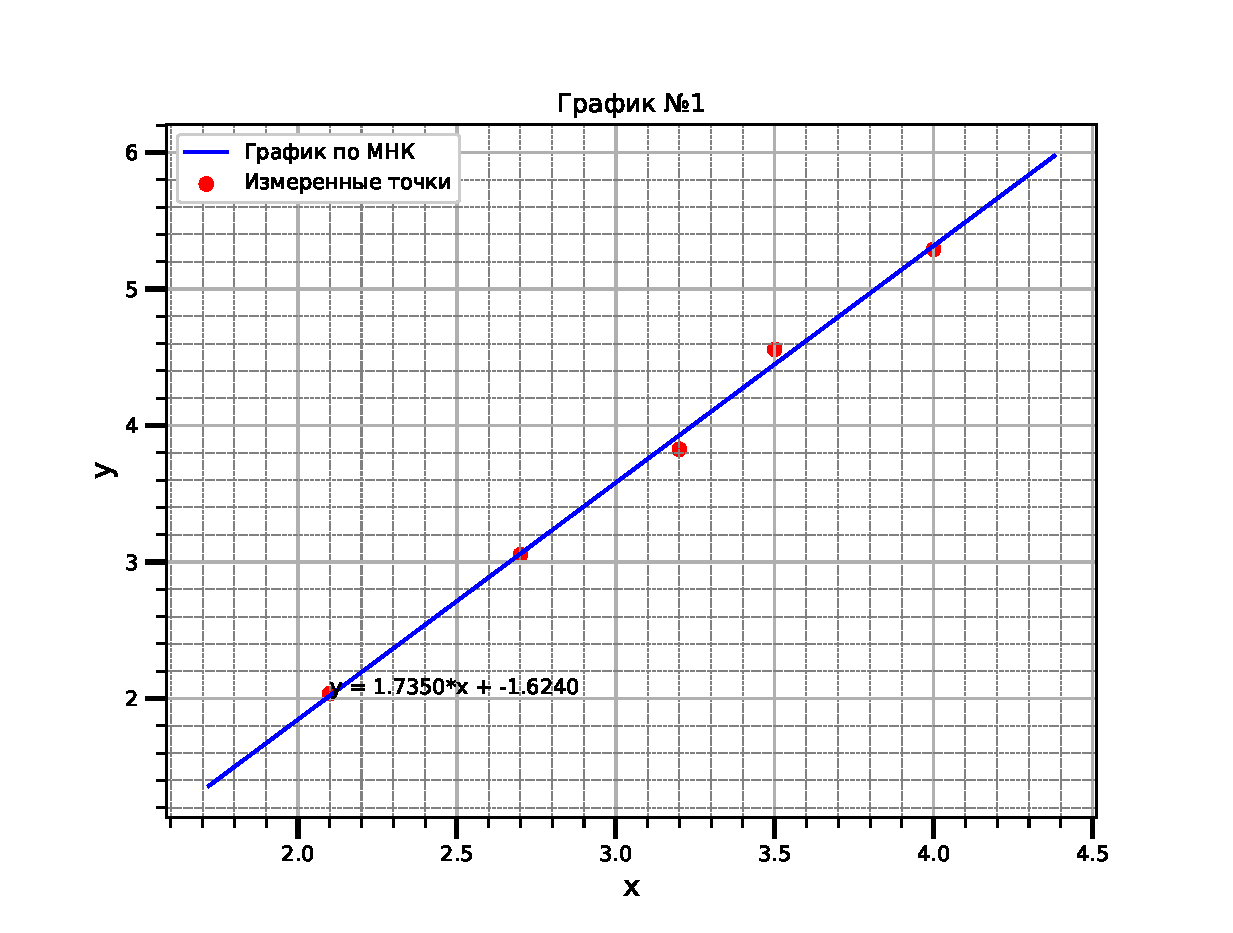
\includegraphics[width=\textwidth]{graph1.eps}
\end{center}

Полученная линейная (вида $y = ax + b$) зависимость: $y =  1.735x - 1.624$\\
$\sigma_a = 0.537$ , $\sigma_b = 0.352$\\
При этой температуре получаем значение коэффициента Джоуля-Томпсона:

$$\frac{\delta T}{\delta P} = 1.735 K/Pa$$

\textbf{При $T = 303$ K:}\\ 

$$
\begin{tabular}{|c|c|c|c|c|c|}
\hline
\multicolumn{6}{|c|}{При $T = 303 K$}\\
\hline
$\Delta P, Pa$&4.0&3.5&3.3&2.7&2.2\\\hline
$\Delta T, K$& 5.088& 4.192& 3.866& 2.768& 1.994\\\hline
\end{tabular}
$$

\begin{center}
    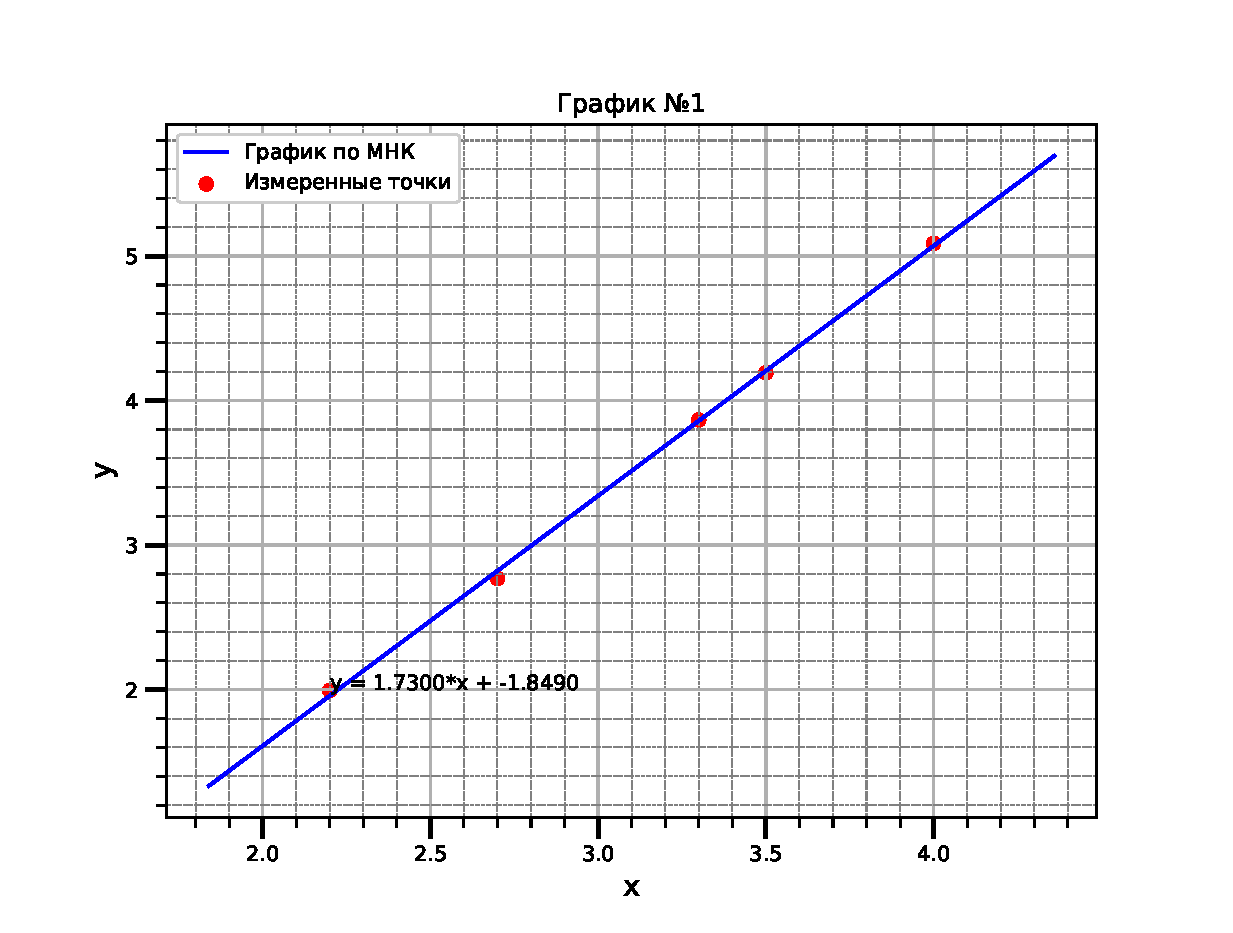
\includegraphics[width=\textwidth]{graph2.eps}
\end{center}

Полученная линейная (вида $y = ax + b$) зависимость: $y =  1.73x - 1.85$\\
$\sigma_a = 0.506$ , $\sigma_b = 0.318$\\

При этой температуре получаем значение коэффициента Джоуля-Томпсона:

$$\frac{\delta T}{\delta P} =  1.73 K/Pa$$

\textbf{При $T = 313$ K:}\\ 

$$
\begin{tabular}{|c|c|c|c|c|c|}
\hline
\multicolumn{6}{|c|}{При $T = 313 K$}\\
\hline
$\Delta P, Pa$&4.1&3.5&3.2&2.7&2.2\\\hline
$\Delta T, K$& 4.95& 3.952& 3.411& 2.87& 1.955\\\hline
\end{tabular}
$$

\begin{center}
    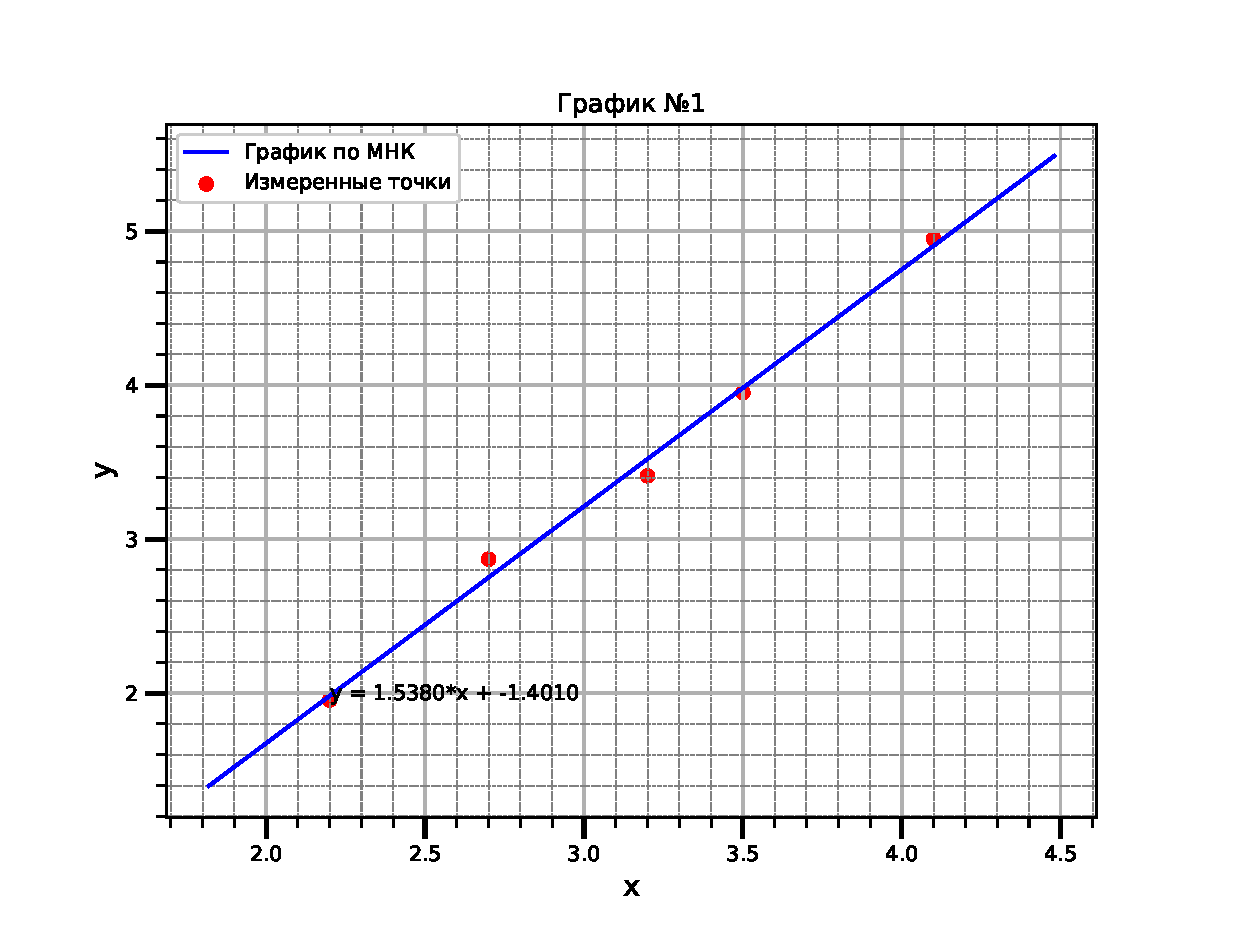
\includegraphics[width=\textwidth]{graph3.eps}
\end{center}

Полученная линейная (вида $y = ax + b$) зависимость: $y =  1.538x - 1.4$\\
$\sigma_a = 0.485$ , $\sigma_b = 0.317$\\

При этой температуре получаем значение коэффициента Джоуля Томпсона:

$$\frac{\delta T}{\delta P} =  1.54 K/Pa$$

\textbf{При $T = 323$ K:}\\ 

$$
\begin{tabular}{|c|c|c|c|c|c|}
\hline
\multicolumn{6}{|c|}{При $T = 323 K$}\\
\hline
$\Delta P, Pa$&4.1&3.5&3.2&2.7&2.2\\\hline
$\Delta T, K$& 4.8& 3.825& 3.442& 2.72& 1.955\\\hline
\end{tabular}
$$

\begin{center}
    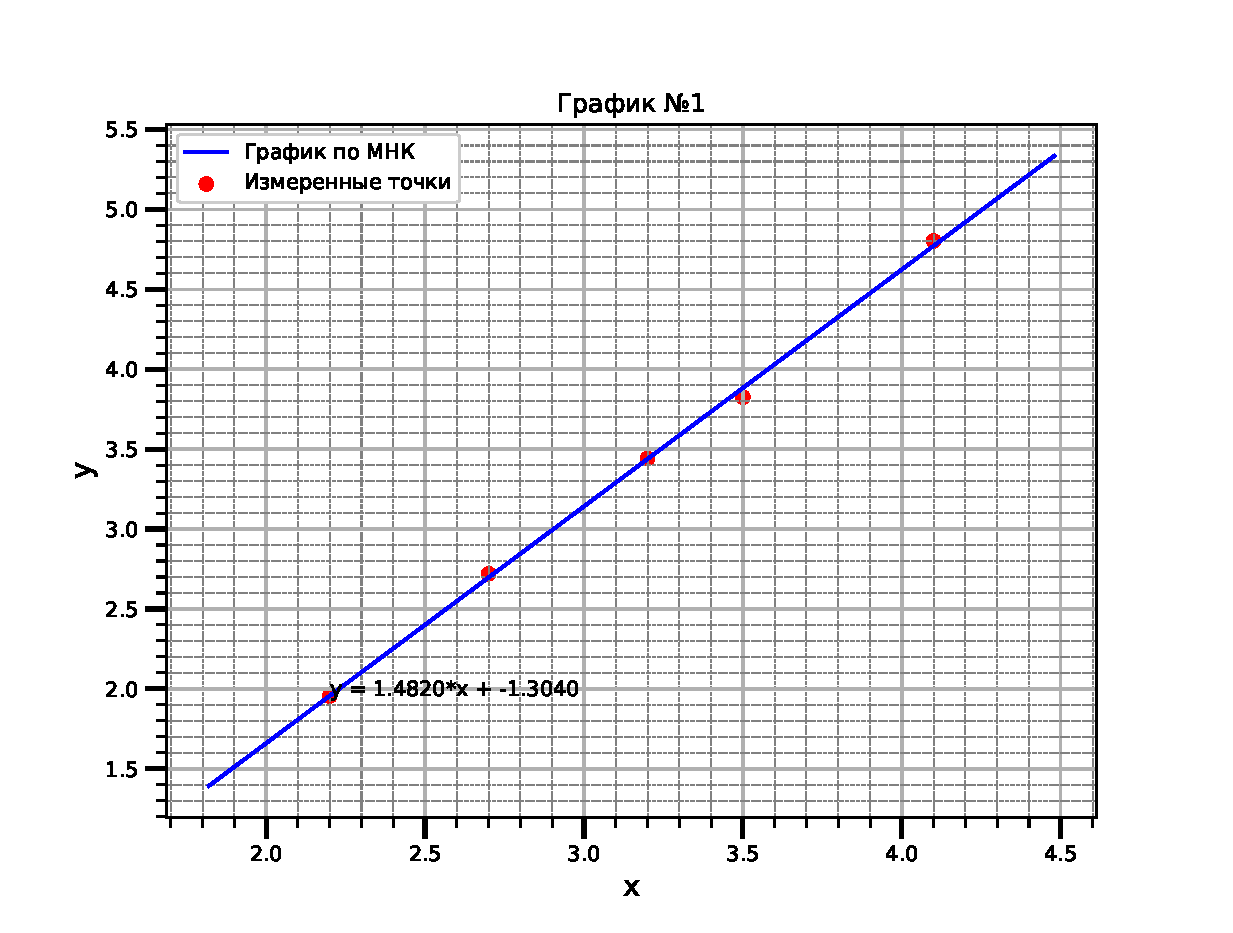
\includegraphics[width=\textwidth]{graph4.eps}
\end{center}

Полученная линейная (вида $y = ax + b$) зависимость: $y =  1.482x - 1.304$\\
$\sigma_a = 0.474$ , $\sigma_b = 0.31$\\

При этой температуре получаем значение коэффициента Джоуля Томпсона:

$$\frac{\delta T}{\delta P} =  1.482 K/Pa$$

\textbf{Построим график $\mu$ от $\frac{1}{T}:$}\\

$$
\begin{tabular}{|c|c|c|c|c|}
\hline
$\frac{1}{T}, 10^{ 3} K^{ 1}$&0.0034&0.003.7&0.0032&0.0031\\\hline
$\mu, K/Pa$& 1.735& 1.73& 1.54& 1.482\\\hline
\end{tabular}
$$

\begin{center}
    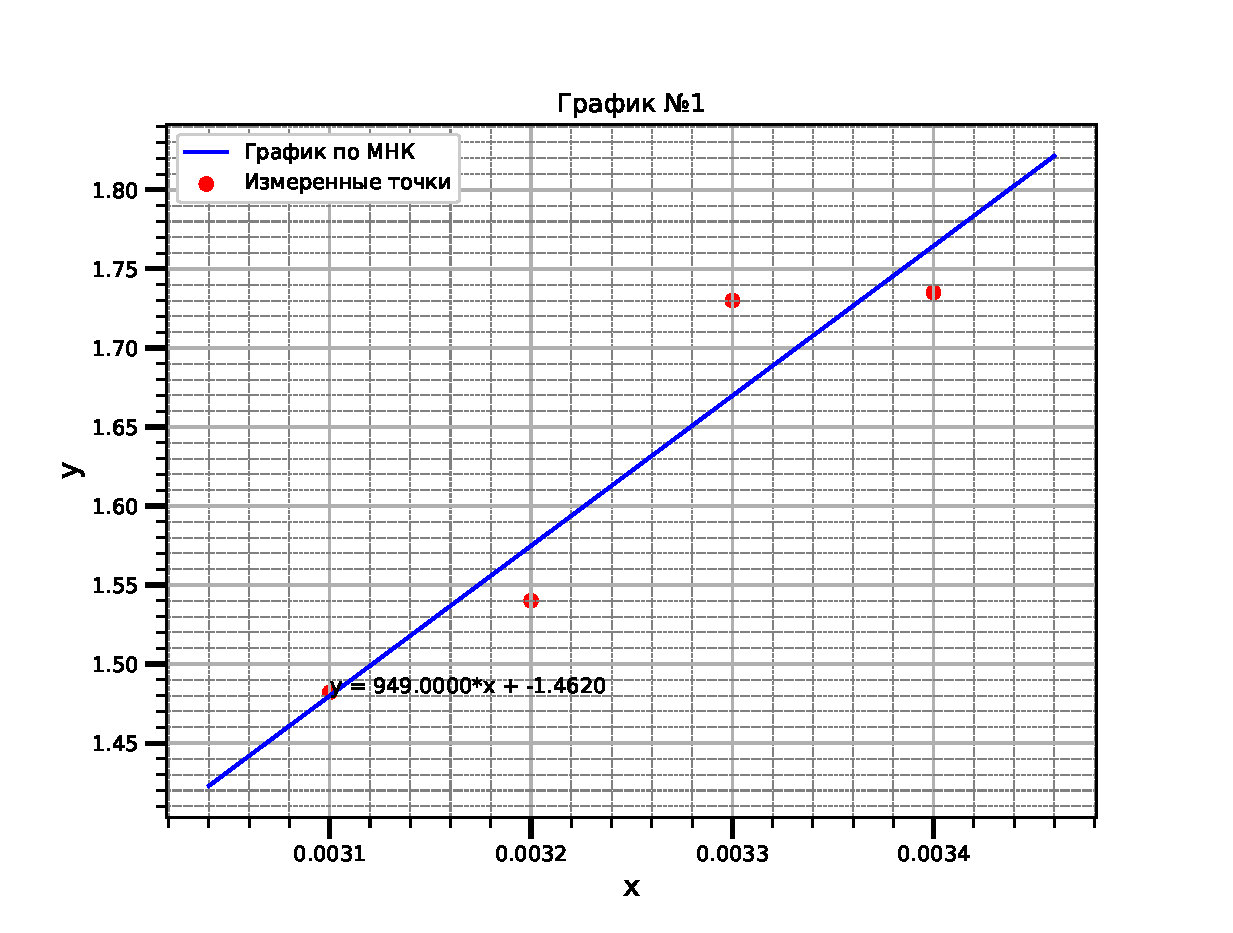
\includegraphics[width=\textwidth]{graph5.eps}
\end{center}

Полученная линейная (вида $y = ax + b$) зависимость: $y =  949x - 1.462$\\
$\sigma_a = 0.006 K^2/Pa$ , $\sigma_b = 6.6$ $10^{-7}$ K/Pa\\

По коэффициентам прямой прямой определим коэффициенты $a$ и $b$ для углекислого газа.\\

Согласно формуле:

$$\mu = \frac{2}{RTC_p} \cdot a  -  \frac{b}{C_p}$$

Из этой зависимости мы можем вычислить значения $a$ и $b$:\\

$$a = 1.46 \frac{\text{н} \cdot \text{м}^4}{mole^2}, b = 54.24 \frac{cm^3}{mole}$$ \\
Коэффициент $b$ достаточно точно совпадает с табличным: $b = 42,8 \frac{cm^3}{mole}$\\
Коэффициент $a$ отличается от табличного $a = 0.36 \frac{\text{н} \cdot \text{м}^4}{mole^2}$ в несколько раз.\\

По пересечению графиком $\mu \left(\frac{1}{T}\right)$ оси абсцисс находим значение температуры
инверсии для углекислого газа:
$$T_{inv} = 649 K$$
Порядок этого значения совпадает с табличным \( T = 2053 K \)\\
\section{Краткие выводы:}
\begin{enumerate}
    \item В ходе работы были экспериментально получены коэффициенты $a$ и $b$ уравнения
    реального газа для углекислого газа. Как сказано выше, коэффициент $b$ достаточно
    точно совпал с табличным в то время как $a$ отличается от табличного в несколько раз.\\
    \item Была также оценена величина $T_{inv}$ инвариантной температуры углекислого газа,
    которая отличается от табличной на порядок.\\
\end{enumerate}



\end{document}
